\documentclass[a4paper,20pt]{article}
\usepackage{amsmath,amssymb,epsf,epsfig,times}
\usepackage{multicol}
\usepackage[all]{xy}
\usepackage{color}
\usepackage{ctex}
\usepackage{subfigure}
\usepackage{url,cite}
\usepackage{tikz}
\usepackage[english]{babel}
\usepackage[utf8]{inputenc}

\usepackage{pdfpages}

%\usepackage{caption}
%
%\usepackage[font=small,labelfont=bf,labelsep=none]{caption}
\usepackage[font=default,labelfont=bf,labelsep=period]{caption}

\usepackage{makecell}
\usepackage{booktabs} %引入三线表
\usepackage{diagbox}
\usepackage{multirow}

\usepackage{fancyhdr}
\usepackage{float}
\usepackage{ulem}

\usepackage{listings}
\usepackage{xcolor}

\usepackage{enumerate}
\lstset{
    basicstyle          =   \sffamily,          % 基本代码风格
    keywordstyle        =   \bfseries,          % 关键字风格
    commentstyle        =   \rmfamily\itshape,  % 注释的风格,斜体
    stringstyle         =   \ttfamily,  % 字符串风格
    flexiblecolumns,                % 别问为什么,加上这个
    numbers             =   left,   % 行号的位置在左边
    showspaces          =   false,  % 是否显示空格,显示了有点乱,所以不现实了
    numberstyle         =   \zihao{-5}\ttfamily,    % 行号的样式,小五号,tt等宽字体
    showstringspaces    =   false,
    captionpos          =   t,      % 这段代码的名字所呈现的位置,t指的是top上面
    frame               =   lrtb,   % 显示边框
}
\lstdefinestyle{Python}{
    language        =   Python, % 语言选Python
    basicstyle      =   \zihao{-5}\ttfamily,
    numberstyle     =   \zihao{-5}\ttfamily,
    keywordstyle    =   \color{blue},
    keywordstyle    =   [2] \color{teal},
    stringstyle     =   \color{magenta},
    commentstyle    =   \color{red}\ttfamily,
    breaklines      =   true,   % 自动换行,建议不要写太长的行
    columns         =   fixed,  % 如果不加这一句,字间距就不固定,很丑,必须加
    basewidth       =   0.5em,
}

\newtheorem{theorem}{Theorem}[section]
\newtheorem{lemma}{Lemma}[section]
\def\proof{\noindent{\it Proof: }}
\def\QED{\mbox{\rule[0pt]{1.5ex}{1.5ex}}}
\def\endproof{\hspace*{\fill}~\QED\par\endtrivlist\unskip}
\newcommand{\re}{\mathbb{R}}
\def\sV{\mathcal{V}}
\def\sS{\mathcal{S}}
\def\sQ{\mathcal{Q}}

\newcommand{\mc}{\mbox{: }}

\newcommand{\normsq}[1]{\left\|#1\right\|^2}
\newcommand{\norm}[1]{\left\|#1\right\|}
%\newcommand{\sgn}[1]{\mbox{sgn}(#1)}
\newcommand{\pde}[2]{\frac{\partial #1}{\partial #2}}
\newcommand{\fundef}[3]{#1:#2\to #3}
\newcommand{\abs}[1]{\left|#1\right|}
\newcommand{\mymatrix}[2]{\left(\begin{array}{#1}#2\end{array}\right)}
\newcommand{\defeq}{\stackrel{\triangle}{=}}
\newcommand{\paren}[1]{\left(#1\right)}
%\theoremstyle{plain} \newtheorem{theorem}{Theorem}
%\theoremstyle{plain} \newtheorem{algorithm}{Algorithm}
\newtheorem{axiom}[theorem]{Axiom}
\newtheorem{definition}[theorem]{Definition}
\newtheorem{assumption}[theorem]{Assumption}
\newtheorem{example}[theorem]{Example}
%\theoremstyle{plain}\newtheorem{lemma}{Lemma}
%\newtheorem{proposition}[theorem]{Proposition}
\newtheorem{remark}[theorem]{Remark}
\newtheorem{corollary}[theorem]{Corollary}

\newcommand{\Acal}{\mathcal{A}}
\newcommand{\Bcal}{\mathcal{B}}
\newcommand{\Ccal}{\mathcal{C}}
\newcommand{\Dcal}{\mathcal{D}}
\newcommand{\Ecal}{\mathcal{E}}
\newcommand{\Fcal}{\mathcal{F}}
\newcommand{\Gcal}{\mathcal{G}}
\newcommand{\Hcal}{\mathcal{H}}
\newcommand{\Ical}{\mathcal{I}}
\newcommand{\Jcal}{\mathcal{J}}
\newcommand{\Kcal}{\mathcal{K}}
\newcommand{\Lcal}{\mathcal{L}}
\newcommand{\Mcal}{\mathcal{M}}
\newcommand{\Ncal}{\mathcal{N}}
\newcommand{\Ocal}{\mathcal{O}}
\newcommand{\Pcal}{\mathcal{P}}
\newcommand{\Qcal}{\mathcal{Q}}
\newcommand{\Rcal}{\mathcal{R}}
\newcommand{\Scal}{\mathcal{S}}
\newcommand{\Tcal}{\mathcal{T}}
\newcommand{\Ucal}{\mathcal{U}}
\newcommand{\Vcal}{\mathcal{V}}
\newcommand{\Wcal}{\mathcal{W}}
\newcommand{\Xcal}{\mathcal{X}}
\newcommand{\Ycal}{\mathcal{Y}}
\newcommand{\Zcal}{\mathcal{Z}}


\def\omegavec{\boldsymbol{\omega}}
\newcommand{\alphabf}{\boldsymbol{\alpha}}
\newcommand{\omegabf}{\boldsymbol{\omega}}
\def\omegavec{\boldsymbol{\omega}}
\newcommand{\taubf}{\boldsymbol{\tau}}
\newcommand{\qbf}{\mathbf{q}}
\newcommand{\ybf}{\mathbf{y}}
\newcommand{\pbf}{\mathbf{p}}
\newcommand{\rbf}{\mathbf{r}}
\newcommand{\ebf}{\mathbf{e}}
\newcommand{\onebf}{\mathbf{1}}
\newcommand{\zerobf}{\mathbf{0}}
\newcommand{\abf}{\mathbf{a}}
\newcommand{\ibf}{\mathbf{i}}
\newcommand{\jbf}{\mathbf{j}}
\newcommand{\kbf}{\mathbf{k}}
\newcommand{\vbf}{\mathbf{v}}
\newcommand{\wbf}{\mathbf{\omega}}
\newcommand{\fbf}{\mathbf{f}}
\newcommand{\zbf}{\mathbf{z}}
\newcommand{\xbf}{\mathbf{x}}
\newcommand{\dbf}{\mathbf{d}}
\newcommand{\Rbf}{\mathbf{R}}
\newcommand{\Tbf}{\mathbf{T}}

\newcommand{\Cbf}{\mathbf{C}}
\newcommand{\Ibf}{\mathbf{I}}
\newcommand{\Pbf}{\mathbf{P}}
\newcommand{\Qbf}{\mathbf{Q}}
\newcommand{\Vbf}{\mathbf{V}}
\newcommand{\Jbf}{\mathbf{J}}
\newcommand{\Xbf}{\mathbf{X}}
\newcommand{\Abf}{\mathbf{A}}
\newcommand{\Kbf}{\mathbf{K}}
\newcommand{\Gammabf}{\boldsymbol{\Gamma}}
\newcommand{\nubf}{\boldsymbol{\nu}}
\newcommand{\xibf}{\boldsymbol{\xi}}
\newcommand{\Xibf}{\boldsymbol{\Xi}}
\newcommand{\Omegabf}{\boldsymbol{\Omega}}


\newcommand{\ubf}{\mathbf{u}}

\newcommand{\lth}{\ell{\text{th}}}
\newcommand{\ith}{i{\text{th}}}
\newcommand{\jth}{j{\text{th}}}
\newcommand{\kth}{k{\text{th}}}
\newcommand{\ip}[2]{\left<#1,~#2\right>}

\newcommand{\OMIT}[1]{}
\title{}
\author{}
\date{}


\pagestyle{fancy}
\fancyhf{}
\chead{\textbf{MATLAB数学建模算法及实例分析}第五章习题答案}
\lhead{魔力铠甲}
\rfoot{Page \thepage}
\begin{document}
\renewcommand{\lstlistlistingname}{代码汇总}
\renewcommand{\lstlistingname}{代码}
\captionsetup[figure]{labelfont={bf},labelformat={default},labelsep=period,name={图}}
\renewcommand\tablename{表}

\begin{itemize}
    \item[1.]
        \par  该问题可以使用图论中的最短路径算法进行求解。
        可以用四维向量来表示状态,其中第一分量表示人,第二分量表示狼,第三分量表示羊,第四分量表示蔬菜;当人或物在此岸时相应分量取1,在对岸时取0。
        \\根据题意,人不在场时,狼要吃羊,羊要吃菜,因此,人不在场时,不能将狼与羊,羊与蔬菜留在河的任何一岸。例如,状态(0,1,1,0)表示人和菜在对岸,这时人不在场,狼吃羊,状态不可行。
        \begin{figure}[h]
            \begin{center}
                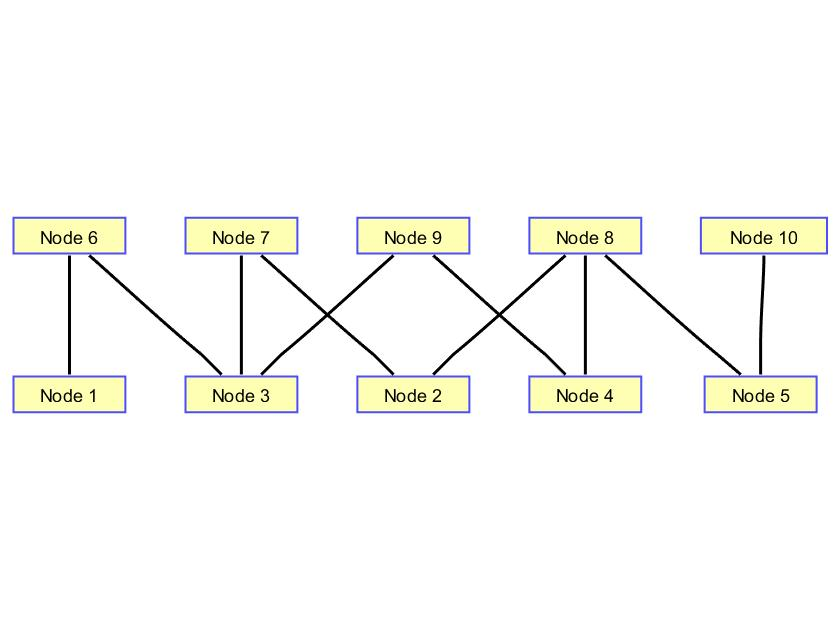
\includegraphics[width=0.80\textwidth]{homework1.jpg}
                \caption{可行状态之间的转移}
            \end{center}
        \end{figure}
        \\故此,可以列出所有可行情况
        \begin{equation}
            \begin{aligned}
                (1,1,1,1),(1,1,1,0),(1,1,0,1),(1,0,1,1),(1,0,1,0), \\
                (0,1,0,1),(0,1,0,0),(0,0,1,0),(0,0,0,1),(0,0,0,0)
            \end{aligned}
        \end{equation}
        \par \noindent 共十种。每一次的渡河行为将改变现有的状态。
        \\现在构造赋权图$G=(V,E,W)$,其中顶点集合$V=\left\{v_1,v_2,\cdots,v_10\right\}$中的顶点(按照上面顺序编号)分别表示上述十个可行状态,当且仅当对应的两个可行状态之间存在一个可行转移时两顶点之间才有边链接,并且对应的权重取1,当两个顶点之间不存在可行转移时,可以把相应权重取为$\infty$。
        \\因此问题变为在图$G$中寻找一条由初始状态(1,1,1,1)出发,经由最小次数转移到达最终状态(0,0,0,0)的最短路径。这就将问题转换为图论中的最短路径问题。
        \\现在规定方向向量运算为
        $$0+0=0,0+1=1,1+0=1,1+1=0$$
        \\这个时候可以根据matlab编程实现(详细见homework1.m)
        \\1     6     3     7     2     8     5    10为路径。经过七次就可以过河。

        \item[2.]
        \par 可以根据本章例题直接进行更改,使用最小生成树代码。(详细见homework2.m)
    \item[3.]
        \par 及$v_i(i=1,2,3,4)$表示第i年年初的时刻,$v_5$表示第四年末的时刻,构造赋权图$G=(V,A,W)$,其中$V=(v_1,\cdots,v_5)$,A为弧的合集,邻接矩阵$W=(w_{ij})_{5\times 5}$,这里$w_{ij}$为$v_i$到$v_j$的费用,例如$w_{12}$为第一年初到第二年初的费用,等于购置费用加维修费用减去机器处理价,$w_{12}=2.5+0.3-2.0=0.8$,则计算可得
        \begin{center}
            $W=\begin{bmatrix}
                    0      & 0.8    & 2      & 3.8    & 6   \\
                    \infty & 0      & 0.9    & 2.1    & 3.9 \\
                    \infty & \infty & 0      & 1.1    & 2.3 \\
                    \infty & \infty & \infty & 0      & 1.4 \\
                    \infty & \infty & \infty & \infty & 0   \\
                \end{bmatrix}$
        \end{center}
        \par  四年内用于更换、购买以及运行维修总费用最盛的问题,归结为求图$G$中从$v_1$到$v_5$的最短路径。
        \\matlab编程实现Dijkstra标号算法(详细见homework3.m)
        \\第二年出第三年初换新,总费用4万元。
    \item[4.]
    \par 应用最大流算法必须是单源和单汇的网络。
    构造一个虚拟的原点$v_x$,由于A,B,C的可供量分别为20,20,100,则弧$v_xA,v_xB,v_xC$上的容量分别为20,20,100,构造一个虚拟的汇点$v_t$,由于市场1、2、3、4的需求量分别为20、20、60、20,市场1,2,3,4分别记为D、F、H、I,则弧$Dv_t,Fv_t,Hv_t,Iv_t$的容量分别为20、20、60、20。
    构造赋权有向图(V,E,W),其中V为顶点集合,E为弧的集合,W为各个弧上的容量所构成的权重矩阵,具体计算时,把顶点$v_x$、A、B、C、D、F、H、I、$v_t$分别编号1~9,从仓库到市场的最大流问问题归结为求$V_x$到$v_t$的最大流,可以使用Ford-Fulkerson算法求最大流。(代码详见homework4.m)
    \item[5.]
    \par 将5个人与5个外语语种分别用点表示,把各个人与懂得的外语语种之间用弧相连。为了求单源和单汇网络的最大流,再加一个虚拟的单源$v_s$,$v_s$与五个人之间个有一条弧,再加一个虚拟的单汇$v_t$,再五个外语语种和$v_t$之间各有一条弧。规定每条弧的容量为1,求出上述网络的最大流数字记为最多能得到招聘的人数。
    计算时把远点$v_s$,甲乙丙丁戊五个人,俄英日德法五个外语语种和汇点$v_t$分别编号为1,2,$\cdots$,12。(代码详见homework5.m)4
    \item[6.]
    \par 可以将这个图形转化成最短路径问题。我们直接构造虚拟单源$S$与虚拟单汇$T$,然后根据最小生成图,我们可以直接得出这个图:
    %  \begin{figure}
    %      \begin{center}
    %          \includegraphics[9.8/textwidth]{imagefile}
    %          \caption{网络图}
    %      \end{center}
    % \end{figure}
\end{itemize}
\end{document}